\documentclass[a4paper]{scrartcl}

\usepackage{mdwlist}
\usepackage{polski}
\usepackage[utf8x]{inputenc}
\usepackage{color}
\usepackage[unicode=true]{hyperref}
\usepackage[table]{xcolor}
\usepackage{listings}
\usepackage{float}
\usepackage{wrapfig}

\usepackage{graphicx}
\graphicspath{{./images/}}
\DeclareGraphicsExtensions{.pdf,.png,.jpg}

\lstset{ %
basicstyle=\footnotesize,       % the size of the fonts that are used for the code
frame=single,                   % adds a~frame around the code
}

% Tego używamy do odnoszenia się do projektu
\newcommand{\omlet}{\textbf{Omelette} }

% Nazwy programów, klas, bibliotek: \textbf
% Nazwy plików, modułów: \textt
% Inne nazwy własne, np. nazwy organizacji: \emph
% listingi:
% \lstinputlisting[language=Python,caption={caption}]{source_filename.py}


\begin{document}
\sloppy

\title{Omelette}
\subtitle{Raport z~projektu}
\author{
  Sławomir Blatkiewicz\and
  Jakub Górniak       \and
  Piotr Piechal       \and
  Bartosz Pieńkowski  \and
  Barnaba Turek       \and
  Michał Zochniak
}
\maketitle

\part{Historia projektu}
\section{Interfejs programu}
Na samym początku projektu, po wybraniu jego tematu, planowaliśmy stworzyć narzędzie obsługiwanie z linii komend do "kompilacji" plików tekstowych w diagramy UML. Mieliśmy również pomysł aby stworzyć moduł do LaTeXa służący do generacji diagramów, jednak szybko go zarzuciliśmy.
Z upływem czasu doszliśmy do wniosku, że łatwiejsze i wygodniejsze w użyciu będzie proste IDE umożliwiające zarówno tworzenie "kodu diagramu" jak i jego "kompilację". W pierwszej wersji okno apliakcji podzielone było na dwie części: część zawierającą kod i diagram. Diagram był statycznym obrazem generowanym na podstawie kodu w sąsiedniej części okna.
Kolejnym krokiem było umożliwienie użytkownikowi przeciąganie elementów na diagramie, który przestał być statyczny. Również okno z kodem otrzymało nową funkcjonalność jaką było podstawowe kolorowanie składni opartej o syntaktykę języka Python. Dodano również przycisk pozwalający na wygenerowanie diagramu w postaci rastrowej i zapisanie jej do pliku.
Następnie okno kodu zostało wypsażone w obsługę składni stworzonego przez nas języka. Kolejnym etapem było wykorzystanie architektury paneli do budowy wewnętrznej struktury okna oraz dodanie panelu obsługi błędów przetwarzania kodu. Dopiero w ostatniej fazie rozwoju aplikacji powstał moduł umożliwiający kompilację kodu do grafiki rastrowej z linii komend.
\section{Język opisu diagramów UML}
Od samego początku zakładaliśmy strukturę języka opartą o system klucz-wartość, którą utrzymaliśmy do końca trwania projektu. Naszym głównym celem było uzyskanie jak największej elastyczności języka, która miała umożliwiać definiowanie własnych elementów diagramów bez konieczności ingerencji w wewnętrzne struktury aplikacji. Zostało to uzyskane przez zastosowanie architektury modułów dołączanych dynamicznie przy uruchomieniu aplikacji. Użytkownik może stworzyć własne moduły, czyli elementy z których mogą składać się diagramy. Przez to możliwości robudowy naszego programu są praktycznie nieograniczone. W tym momencie użytkownik nie jest związany z notacją UML. Dopisując własne moduły można adaptować naszą aplikację np. do tworzenia diagramów BPMN.
W obecnej formie możliwa jest również walidacja kodu poddawanego kompilacji oraz zwrócenie wykrytych błędów wraz z numerami linii w których wystąpiły oraz prostą diagnostyką. Użytkownik w momencie kompilacji otrzymuje informację zwrotną na temat popełnionych błędów w konstrukcji kodu diagramu, które nie zawsze muszą być widoczne wprost.
\section{Sposób przyłączania relacji do obiektów}
Istotnym z punktu widzenia projektu architektury aplikacji zagadnieniem jest sposób w jaki relacje są podłączane do obiektów na diagramie. Na samym początku planowaliśmy by obiekty posiadały zbiór punktów na obrysie jego reprezentacji, do których relacja może zostać przyłączona. Takie rozwiązanie jednak stwarzało pewne problemy. Po pierwsze nie byliśmy w stanie z góry przewidzieć ile takich punktów na każdej krawędzi należy wyznaczyć aby wszystkie podłączone relacje wyglądały naturalnie. Natomiast zmiana zbioru tych punktów przy już istniejących dołączonych relacjach powodowałaby konieczność przeliczania ich położenia i przesuwania dołączonych relacji.
Rozwiązanie na które zdecydowaliśmy się ostatecznie jest nieporównywalnie prostsze zarówno ideowo jak i w implementacji. Mianowicie każdy obiekt ma jeden punkt, do którego przyłączane są wszystkie relacje, umieszczony w jego centrum. Takie rozwiązanie wymusiło na nas rozwiązanie problemu przesłaniania relacji przez reprezentację graficzną obiektu. Realizowane jest to poprzez znajdowanie przecięć (w geometrycznym znaczeniu) reprezentacji graficznej z relacją, a następnie przycinaniu linii ją symbolizującej.
\section{Integracja}
Na samym początku projektu nie było wyraźnego podziału funkcjonalności aplikacji pomiędzy członków zespołu. Każdy tworzył fragmenty które stanowiły odrębne byty, między którymi nie istniały ustalone interfejsy komunikacyjne. Jednak w momencie w którym byliśmy gotowi na zapewnienie podstawowej funkcjonalności pierwszej wersji aplikacji okazało się, że doskonale działające w odosobnieniu moduły nie mają wspólnych interfejsów. Co więcej stworzenie ich nie było trywialną sprawą. Pomimo tego powstała pierwsza, i choć bardzo niedoskonała, to działająca wersja aplikacji zapewniająca podstawową funkcjonalność.
Ponieważ wersja ta, ze względu na wspomniane problemy, była bardzo niedoskonała pod względem programistycznym, zdecydowaliśmy się na daleko idącą refaktoryzację kodu wraz z redefinicją kanałów komunikacyjnych. Dzięki temu krokowi powstała wersja aplikacji cechująca się pełną integracją modułów, jasno wyznaczonymi granicami funkcjonalności oraz jednoznacznie określonymi interfejsami między nimi. Także pojawiły się wyraźne podziały odpowiedzialności za poszczególne części aplikacji pomiędzy członków zespołu.
Od tej pory praca nad rozwojem aplikacji była o wiele łatwiejsza i przebiegała bez większych problemów. Każdy z programistów rozwijał kod, który bardzo dobrze znał z poprzedniego etapu rozwoju aplikacji, co znacznie przyspieszyło pracę i współpracę. Jednak co ważniejsze, od tego czasu aplikacja jest w pełni zintegrowana, a poprawki wprowadzane przez programistów nie zaburzały tej integralności. Praktycznie w każdej chwili aplikacja była gotowa do uruchomienia.
Wraz z tą zmianą, nadszedł czas wzajemnego testowania własnego kodu. Ponieważ aplikacja po wprowadzeniu zmian nie przestawała działać, wszyscy programiści dysponujący najnowszą wersją uruchamiając ją, chcąc czy nie chcąc, testowali kod nie tylko swój ale także innych członków zespołu. Od tej pory zaczęliśmy wzajemnie zgłaszać sobie zauważone usterki co drastycznie przyspieszyło tempo ich znajdowania.

\section{Zarządzanie projektem}

Ze względu na rozwojowy charakter projektu i~niedookreśloną formę produktu
końcowego do prowadzenia projektu starano się zaadaptować zwinną metodykę
\emph{Scrum}.
Jako długość sprintu przyjęto stały okres dwóch tygodni, po upłynięciu których,
począwszy od ostatniego tygodnia pierwszego semestru, sporządzany był zbiorowy
raport relacjonujący pracę wykonaną przez każdego członka zespołu.

W~początkowej fazie trwania projektu przed rozpoczęciem każdego sprintu
ustalane były zadania, które następnie podlegały estymacji przy użyciu techniki
o~nazwie \emph{Planning Poker}, w~której udział brali wszyscy członkowie
zespołu.
Ustalanie terminarza sprintów, zarządzanie zadaniami (w~tym przypisywanie
ich konkretnym osobom oraz śledzenie stanu wykonania), jak również
monitorowanie kondycji całego projektu możliwe było dzięki wykorzystaniu
serwisu \emph{Scrum'd}.

\begin{figure}[ht]
	\centering
		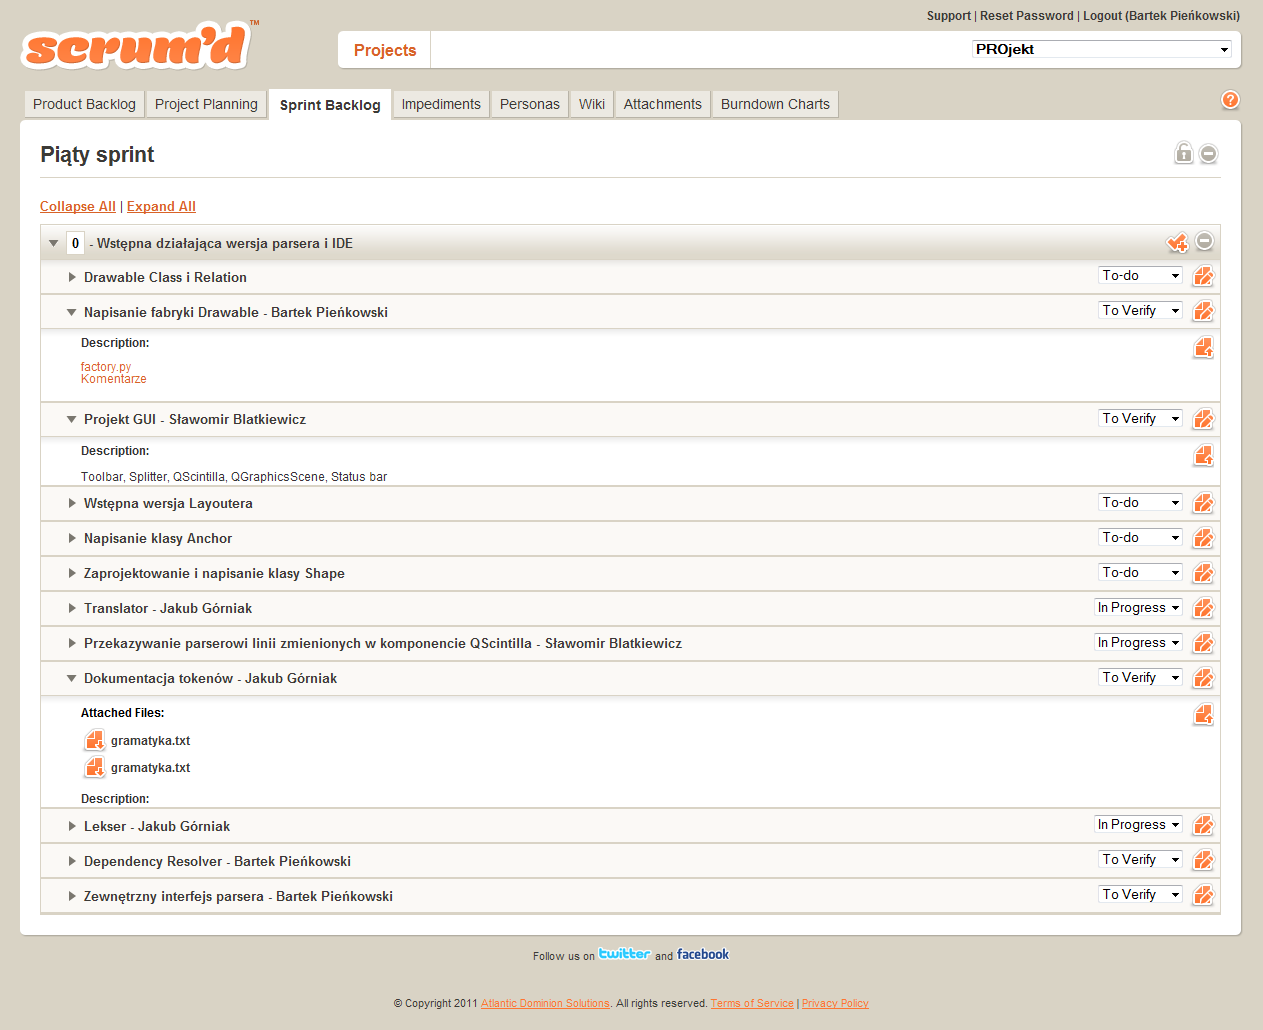
\includegraphics[scale=0.3]{scrumd}
	\caption{Wygląd listy zadań w~serwisie \emph{Scrum'd}}
	\label{fig:scrumd}
\end{figure}

Dążąc do zapewnienia wysokiej jakości tworzonego kodu każdy nowo powstały
fragment programu, przed dostaniem się do głównego repozytorium, weryfikowany
był przez kierownika projektu i~pozostałych członków zespołu w~celu wskazania
błędów i~odnotowania ewentualnych uwag. Komentowanie kodu z~dokładnością do
pojedynczej linii możliwe było dzięki bogatej funkcjonalności serwisu
\emph{GitHub}.

W~miarę upływu czasu każdy z~członków zespołu zaczął zajmować się określonym
obszarem projektu, dzięki czemu podział zadań stał się oczywisty. Podczas
wzmożonej pracy nad stworzeniem demonstracyjnej wersji programu większość zadań
przerodziła się w~drobne poprawki, czego efektem była (prawdopodobnie
niesłuszna) rezygnacja z~dalszej estymacji zadań.

W~celu przyspieszenia procesu integracji zorganizowano w~tamtym okresie kilka
spotkań w~laboratorium 225, na których stawiła się większość członków zespołu.
Zalety takiego sposobu pracy (szybkie tempo, ułatwiona komunikacja wewnątrz
zespołu) były niepodważalne. W~efekcie proces pełnej integracji kodu
zakończył się sukcesem.

Nowy sposób pracy narzucił wymóg korzystania z~bardziej odpowiedniego narzędzia
do zarządzania nim, zrezygnowano więc z~używania serwisu \emph{Scrum'd} na rzecz
o~wiele prostszego w~założeniach i~obsłudze serwisu \emph{Checkvist}, będącego
interaktywną listą zadań dającą możliwość współtworzenia wszystkim członkom
zespołu. Zakres możliwości tego narzędzia obejmuje dodawanie i~usuwanie zadań,
oznaczanie ich jako wykonanych, komentowanie oraz ustalanie terminarza.

\begin{figure}[ht]
	\centering
		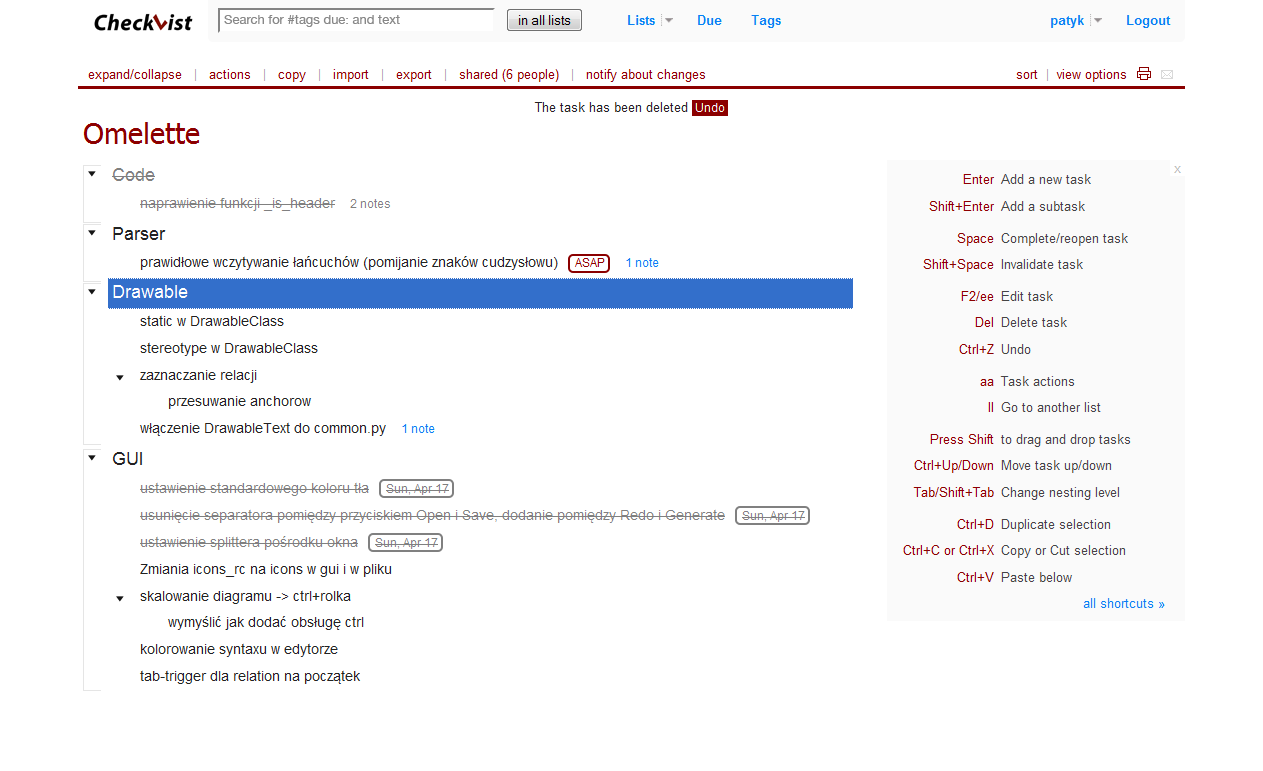
\includegraphics[scale=0.3]{checkvist}
	\caption{Wygląd listy zadań w~serwisie \emph{Checkvist}}
	\label{fig:checkvist}
\end{figure}

W~końcowej fazie projektu zaczęto wykorzystywać nowy \emph{issue tracker}
udostępniony w~ramach serwisu \emph{GitHub}. Zarządzanie zadaniami przy pomocy
tego narzędzia obejmowało m.in. przypisywanie ich konkretnym osobom, ustalanie
kamieni milowych i~dodawanie etykiet. Korzyścią wynikającą z~jego używania była
jawność zadań i~osób za nie odpowiedzialnych, jak również możliwość zamykania
wykonanych zadań udostępniona wszystkim członkom zespołu.

\begin{figure}[ht]
	\centering
		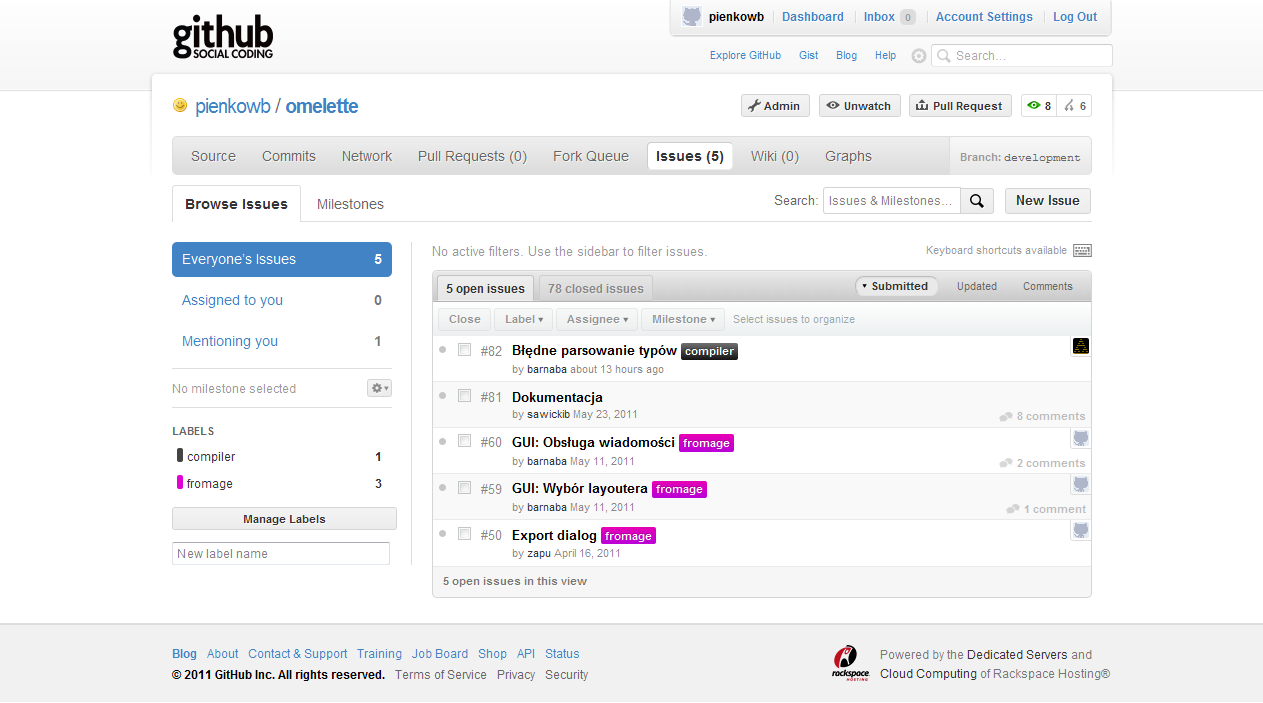
\includegraphics[scale=0.3]{github-issues}
	\caption{Nowy \emph{issue tracker} oferowany przez serwis \emph{GitHub}}
	\label{fig:github-issues}
\end{figure}

Oceniając projekt z~perspektywy kierownika można stwierdzić, iż niewątpliwą
trudnością w~zarządzaniu zespołem były opóźnienia w~dostarczaniu kodu przez
niektórych członków zespołu oraz problemy z~egzekwowaniem przydzielonych zadań.
Ostatecznie udało się w~dużym przybliżeniu zrealizować zamierzoną
funkcjonalność (która nie została przecież dokładnie sprecyzowana), więc
projekt nie okazał się porażką. Z~drugiej strony, mimo negatywnego nastawienia
niektórych członków zespołu, można było utrzymać bardziej wydajne tempo pracy.


\part{Podział obowiązków}
\section{Sławomir Blatkiewicz}
W czasie trwania projektu zajmowałem się głównie warstwą Graficznego Interfejsu Użytkownika. Wraz z kolegą sprawdzalismy możliwosci biblioteki graficznej PyQt które można spożytkować w naszej aplikacji. Szczególną moją uwagę na tym etapie przykuwał komponent edytora kodu źródłowego. Badałem możliwosć generowania diagramu w czasie rzeczywistym, już de facto podczas wprowadzania kodu w edytorze(czego nie udało się osiągnąć). Pomagałem również przy panelu diagramów. Do moich obowiązków należało również przystosowanie interfesju zewnętrznego do zmian jakie występowały w innych modułach. 
\section{Piotr Piechal}
W projekcie zajmowałem się layouterem diagramów. Zarówno wyborem algorytmów jak i ich implementacją oraz projektowaniem struktur wykorzystywanych przy ich realizacji.
Na początku projektu wraz z kolegami opracowaliśmy interfejs modułu realizującego zadania layoutera. Następnie rozpocząłem poszukiwanie algorytmów zapewniających tę funkcjonalność. W ich wyniku stworzyłem opracowanie algorytmów, które nadają się do naszych zastosowań. Były to głównie algorytmy grawitacyjne lub sprężynowe. Następnie wspólnie z kolegami ustaliliśmy kolejność w jakiej będziemy chcieli implementować wybrane algorytmy.
W pierwszej kolejności opracowałem, zaimplementowałem i zoptymalizowałem algorytm rozkładu kołowego. Działa rozkładając wierzchołki diagramu na okręgu minimalizując liczbę przecięć krawędzi poprzez umieszczanie sąsiadujących wierzchołków blisko siebie. Algorytm ten daje doskonałe wyniki w przypadku grafów gęstych o niewielkiej liczbie wierzchołków.
Po zakończeniu fazy testów przeszedłem do implementacji pierwszego z algorytmów wytypowanych do umieszczenia w naszym projekcie - algorytmu Eadesa. Pseudokod algorytmu był bardzo ogólny i wymagał w dużej mierze własnej interpretacji. Po zaimplementowaniu go okazało się, że nie działa poprawnie. Po wielu nieudanych próbach poprawienia efektów jego działania zdecydowaliśmy się skorzystać z gotowej implementacji z biblioteki Graphviz.
Niestety spędziłem tak wiele czasu na próbach poprawienia wyników algorytmu że nie wystarczyło mi czasu na implementację żadnego innego algorytmu z naszej listy.
Planowałem również zaimplementować algorytm grupujący niektóre węzły, których sposób rozłożenia jest z góry znany (np. generalizacja). Algorytm rozkładania miał operować zarówno na pojedynczych wierzchołkach jak i na ich grupach. Niestety tego pomysłu również nie udało się zrealizować ze względu na brak czasu.

\section{Bartosz Pieńkowski}
Poza pracą wynikającą z~pełnienia obowiązków kierownika projektu, skupiającą się na administrowaniu głównym repozytorium, sporządzaniu raportów i~dbaniu o~równy przydział pracy, aktywnie uczestniczyłem w~podejmowaniu wszystkich decyzji projektowych i~tworzeniu architektury programu. Miałem duży wpływ na ostateczny wygląd składni języka -- wiele z~pomysłów, które zaproponowałem, miało przełożenie na obowiązujący projekt gramatyki.

Samodzielnie zaprojektowałem moduł \texttt{code}, odpowiedzialny za wstępne dzielenie kompilowanego kodu na części zawierające pojedyncze obiekty. Ostatecznie potencjał tego modułu nie został w~pełni wykorzystany, gdyż kod za każdym razem kompilowany jest w~całości, a~napisana przeze mnie klasa \textbf{Code} pozwalała ustalić, które obiekty uległy zmianie, pod warunkiem aktualizowania kodu w~trakcie edycji.

Odpowiadam także za pierwszą wersję klasy \textbf{DrawableFactory}, która zapewniała dynamicznie ładowanie klas z~konkretnych modułów na podstawie typu obiektu UML. Zaletą takiego rozwiązania była możliwość rozszerzania języka o~kolejne elementy bez zmian w~module rysującym. Klasa ta została później udoskonalona przez innego członka zespołu i~stała się częścią modułu \texttt{diagram}, w którym przeprowadziłem gruntowną modyfikację zmieniając architekturę modułów z~klasami rysującymi.

Kolejnym moim dokonaniem jest klasa \textbf{Compiler}, której zadaniem jest przeprowadzanie kolejnych etapów kompilacji począwszy od parsowania, a na walidacji kończąc. Integruje ona kilka innych klas -- m.in. klasę \textbf{DependencyResolver} realizującą rozwiązywanie relacji dziedziczenia pomiędzy obiektami oraz klasę \textbf{Validator} odpowiedzialną za weryfikację zdefiniowanych kluczy obiektu na podstawie danych walidacji. W~przypadku obu tych klas miałem ogromny wpływ na ich projekt oraz implementację.

\section{Barnaba Turek}
W początkowej fazie projektu zajmowałem się głównie planowaniem architektury i sposobu działania kompilatora.
Potem zacząłem implementować klasy, które miały leżeć u podstaw tej architektury (Takie jak \textbf{UMLObject}).
Na tym etapie projektu znacząca część mojej aktywności polegała na pomaganiu niektórym kolegom w opanowaniu stosowanych technologii (głównie obsługi repozytorium) i czytaniu książki ``Dive into Python''.
Zajmowałem się też zarządzaniem repozytorium --- tworzeniem struktury katalogów, paczek, wybieraniem i sprawdzaniem możliwości frameworków, używanych do testowania.

W dalszych etapach projektu zajmowałem się też modułem common, który zawierał generyczne klasy, na których miały bazować konkretne klasy środowiska graficznego reprezentujące obiekty na diagramie.
Wprowadzałem też drobne zmiany w modułach \emph{actions}, \emph{code}, \emph{parser}, \emph{layouter}, \emph{logging}.
Moduły \emph{common} i \emph{uml} (a także ich testy) wymagały wielokrotnego poprawiania.
Dzięki temu zyskałem praktykę w pisaniu dobrych (nie specyficznych) testów jednostkowych.
%\href{http://dl.dropbox.com/u/10621643/actually.png}{Mimo tej praktyki, jak ktos cos zmieni w w/w modułach, to będzie musiał przepisać wszystkie testy}

\section{Michał Zochniak}
W projekcie zajmowałem się projektowaniem oraz implementacją warstwy aplikacji służącej do rysowania diagramów. Analizowałem oraz podejmowałem decyzje na temat komunikacji modułów kompilatora, rysowania oraz GUI. Przez cały czas życia projektu utrzymywałem moduł tworzenia diagramów z linii komend który wymagał częstej refaktoryzacji ze względu na dynamikę zmian w innych modułach, z których korzysta.
Podczas projektu mocno podniosłem swoją wiedzę z zakresu Pythona oraz biblioteki Qt. Cały czas szukałem nowych rozwiązań dla istniejących (oraz tych które miały dopiero się ukazać) problemów. Jedyną niepokonaną przeszkodą okazała się generacja diagramów z poziomu konsoli w środowisku bez X-Server. Po wielu dniach poszukiwań oraz nieprzespanych nocy spędzonych na debugowaniu, doszedłem do wniosku, że jedyną możliwością jest użycie zewnętrznej biblioteki do rysowania czcionek - Qt polega na X-Serverze w sprawach czcionek. Uznaliśmy, że koszt jest większy niż zysk i zrezygnowaliśmy z możliwości generowania diagramów w środowisku bez ,,X-ów''.

\part{Opis architektury aplikacji}
\section{Opis i~uzasadnienie technologii}
\subsubsection{Python}

\begin{wrapfigure}{r}{0.22\textwidth}
  \begin{center}
    
\includegraphics[width=0.2\textwidth]{python}
  \end{center}
\end{wrapfigure}
Jako język programowania wybraliśmy język \textbf{Python}.

\textbf{Python} to interpretowany język ogólnego zastosowania, pozwalający programować na wysokim poziomie abstrakcji.
Język oparty jest na wielu paradygmatach programowania: programowaniu obiektowym, programowaniu funkcjonalnym i programowaniu imperatywnym.
Typowanie w \textbf{Pythonie} jest dynamiczne, a typy są mocne.
Zarządzanie pamięcią odbywa się dynamicznie.

Interpretery \textbf{Pythona} dostępne są na wszystkie popularne systemy operacyjne, wiele z nich jest otwartym oprogramowaniem.
Sama specyfikacja języka zarządzana jest przez \emph{Python Software Foundation}~--- niezależną organizację non-profit.

Głównym powodem, dla którego zdecydowaliśmy się na język \textbf{Python} to jego popularność.
Język ten ma opinię języka o bardzo dobrej dokumentacji.
Popularność wpływa także na dostępność dużej ilości otwartych bibliotek, z których wiele jest dojrzałych i wysokiej jakości.

Wielu z nas korzysta na co dzień z systemu GNU/Linux, gdzie wiele aplikacji jest napisanych w języku \textbf{Python}.
Znajomość języka \textbf{Python} pozwoliłaby nam więc robić zmiany w aplikacjach, z których korzystamy na co dzień.

Jednym z powodów, dla którego wybraliśmy język \textbf{Python} był także fakt, że nikt z nas go nie znał.
Wybranie nieznanego dotąd języka miało sprawić, że projekt będzie bardziej interesujący oraz zwiększyć kompetencje zawodowe członków zespołu
\footnote{W razie gdyby projekt nie okazał się hitem na miarę Napstera i musielibyśmy się jeszcze kiedykolwiek starać o pracę.}
.

\subsection{pyparsing}
\textbf{Pyparsing} to jedna z bibliotek, które skłoniły nas do wybrania języka \textbf{Python} do realizacji tego projektu.
Biblioteka \textbf{Pyparsing} to otwarte oprogramowanie.

Biblioteka pozwala w prosty sposób zbudować rekursywny analizator składniowy zstępujący.
Gramatyka, pod kątem której analizowany ma być plik źródłowy, określana jest za pomocą języka \textbf{Python} w plikach źródłowych projektu (W naszym przypadku w pliku \texttt{lexer.py}).
Pyparsing jest używany w takich projektach jak Django, pydot czy Graphite.

Parsowaną gramatykę opisuje się tworząc odpowiednie obiekty.
Obiekty te mogą reprezentować symbole terminalne (wyrażenia regularne, zestawy znaków, pojedyncze znaki lub ich ciągi) lub ich produkcje.
Każdemu obiektowi można przypisać akcję, która zostanie wykonana, gdy dany symbol zostanie wczytany.

\subsection{Qt i pyQt}
\begin{wrapfigure}{r}{0.22\textwidth}
  \begin{center}
    
\includegraphics[width=0.2\textwidth]{qt}
  \end{center}
\end{wrapfigure}
\textbf{Qt} to zestaw przenośnych bibliotek i narzędzi programistycznych dedykowanych do języków \emph{C++} i \emph{Java}.
Pozwala budować graficzne interfejsy użytkownika w sposób zorientowany obiektowo.

Środowisko Qt to otwarte oprogramowanie.
Środowisko dostępne jest na platformy \emph{X11}, \emph{Windows}, \emph{Mac OS X}, \emph{Haiku}, oraz na urządzeniach przenośnych opartych na Linuksie, \emph{Windows CE} i~\emph{Symbian}.

Biblioteki \textbf{Qt} oprócz obsługi interfejsu użytkownika, zawierają także niezależne od platformy systemowej moduły obsługi procesów, plików, sieci, grafiki trójwymiarowej (OpenGL), baz danych (SQL), języka XML, lokalizacji, wielowątkowości, zaawansowanej obsługi napisów oraz wtyczek.

Dzięki bibliotece \textbf{pyQT} mogliśmy skorzystać ze środowiska \textbf{Qt} z poziomu języka \textbf{Python}.

Do graficznego projektowania interfejsu użytkownika użyliśmy programu \textbf{Qt Designer}.

Zdecydowaliśmy się na środowisko \textbf{Qt} ze względu na jego popularność, dostępność na platformy mobilne (wierzymy, że znajomość tego środowiska będzie dla nas cenna w przyszłości), fakt że jest to środowisko w pełni zorientowane obiektowo, oraz dostępność dojrzałej biblioteki do języka \textbf{Python}.

\subsection{Nosetests}
\textbf{Nosetests}, to biblioteka, której używaliśmy do testowania wytwarzanego przez nas oprogramowania.
Biblioteka bazuje na module \texttt{unittest} dostarczanym w standardowej bibliotece języka \textbf{Python}.

Głównym powodem, dla którego zdecydowaliśmy się na korzystanie z tej biblioteki jest jej zdolność do automatycznego dodawania potrzebnych ścieżek.
Ta cecha jest niezbędna do uruchamiania testów bez IDE, a alternatywą jest dopisanie kilku linii, ustawiających ścieżki na prawidłowe w każdym teście.

Ponadto \textbf{Nosetests} udostępnia wiele rozszerzeń, ułatwiających pisanie testów, takich jak generatory testów.

\subsection{Git i Github}
\begin{wrapfigure}{r}{0.22\textwidth}
  \begin{center}
    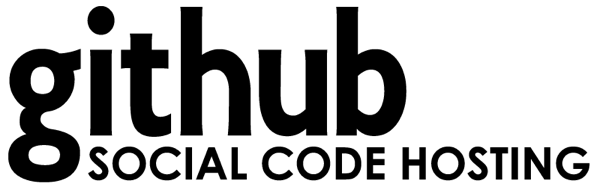
\includegraphics[width=0.2\textwidth]{github}
    
\includegraphics[width=0.2\textwidth]{git}
  \end{center}
\end{wrapfigure}
\textbf{Git} to otwarty rozproszony system kontroli wersji.
Pozwala na łatwe tworzenie i łączenie gałęzi rozwoju projektu, szybkie przemieszczanie się pomiędzy wersjami i sprawdzanie różnic pomiędzy nimi.
\textbf{Git} jest stosowany w takich projektach, jak jądro systemu Linux i umożliwia bardzo wiele (nawet w stosunku do innych nowoczesnych rozproszonych systemów kontroli wersji).
Niestety, powoduje to, że nie jest to system łatwy w nauce.

Zdecydowaliśmy się na system \textbf{Git}, ze względu na doskonały serwis \emph{Github}\footnote{\url{http://github.com}}

Serwis \emph{Github} posłużył nam nie tylko, jako przestrzeń do współdzielenia kodu.
Serwis ten udostępnia wiele narzędzi, które były bardzo przydatne w czasie prac nad projektem.
Korzystaliśmy z wykresów, które pomagały się zorientować, który członek zespołu co robi.
Inna przydatna opcja, z której korzystaliśmy, aby zapewnić wysoką jakość kodu, to komentowanie kodu napisanego przez innych.
Od kiedy został wprowadzony ulepszony system zadań (\emph{Issues 2.0}), korzystaliśmy z niego w celu przechowywania wymagań i komunikacji z opiekunem projektu.

Ponadto serwis pozwala na automatyczne powiadamianie o nowych zmianach w projekcie na kanale IRC, co było bardzo pomocne~--- motywowało do przeglądania kodu innych i usprawniało integrację.

\subsection{Inne narzędzia}
\subsubsection{Zintegrowane środowisko programistyczne}
W zespole nie zostało ustalone żadne środowisko programistyczne.
Część członków zespołu używała środowiska \emph{Eclipse}, część \emph{Netbeans}.

Niektórzy członkowie zespołu tworzyli kod za pomocą zwykłych edytorów tekstowych.

\subsubsection{Kanały komunikacji}
Głównymi kanałami komunikacji wewnątrz zespołu były rozmowy w rzeczywistości i na kanale IRC.

Ponadto, przez pewien czas korzystaliśmy z serwisu \emph{Scrumd}\footnote{\url{http://scrumd.com}}, służącego do zarządzania projektami prowadzonymi w metodyce Scrum.
Głównym zastosowaniem tego narzędzia było przechowywanie wymagań.
Wprowadzenie systemu \emph{issues 2.0} w serwisie \emph{Github} sprawiło, że serwis przestał być przydatny.

Korzystaliśmy także z serwisu \emph{piratepad}\footnote{\url{http://piratepad.net}}.
Serwis ten pozwala na jednoczesną edycję plików tekstowych i łatwe dzielenie się nimi.
Z serwisu korzystaliśmy we wczesnych wersjach projektu, kiedy ustalaliśmy ogólne cele i założenia.


\section{Diagramy Klas}
\begin{figure}
  \begin{center}
    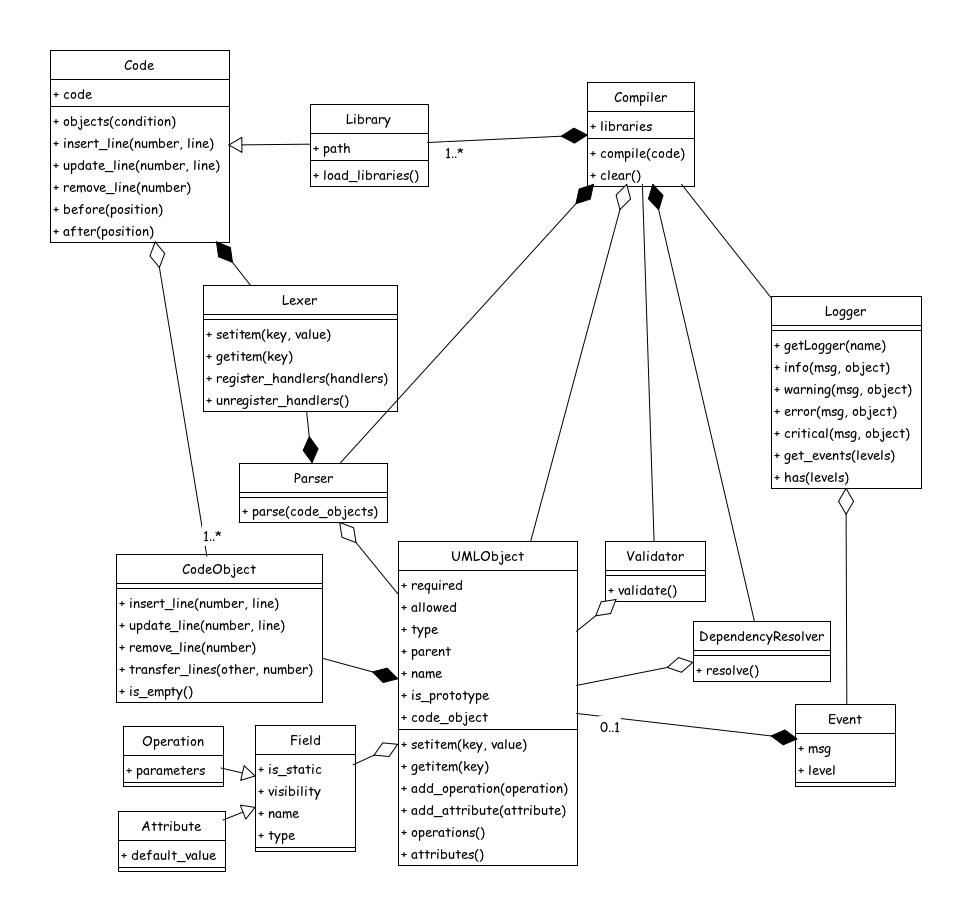
\includegraphics[width=\textwidth]{compiler}
  \end{center}
  \caption{Diagram klas modułu \texttt{compiler}}
\end{figure}

\begin{figure}
  \begin{center}
    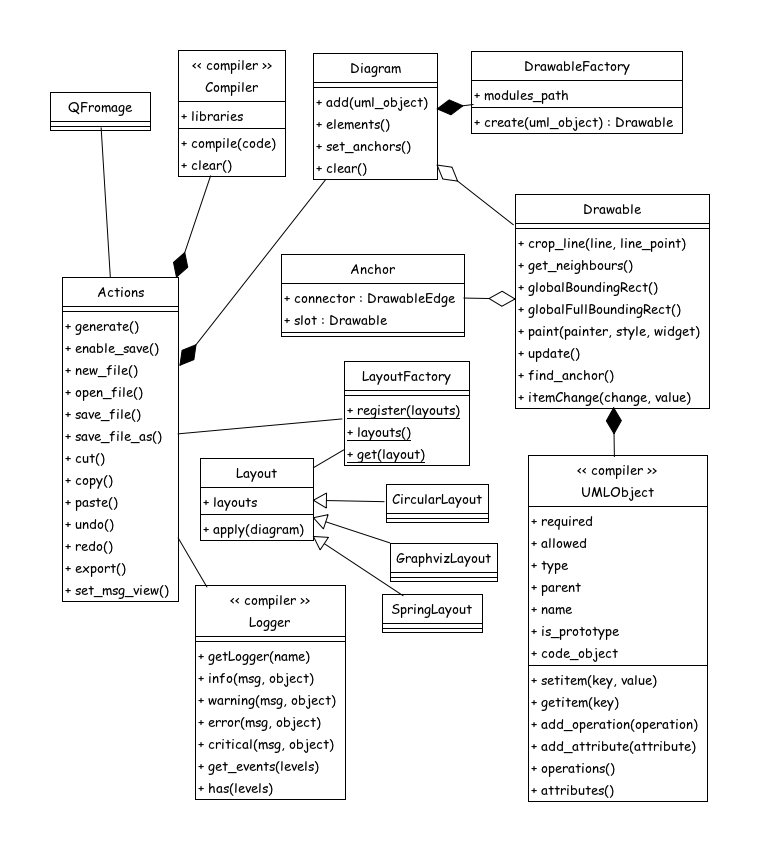
\includegraphics[width=\textwidth]{fromage}
  \end{center}
  \caption{Diagram klas modułu \texttt{fromage}}
\end{figure}

\begin{figure}
  \begin{center}
    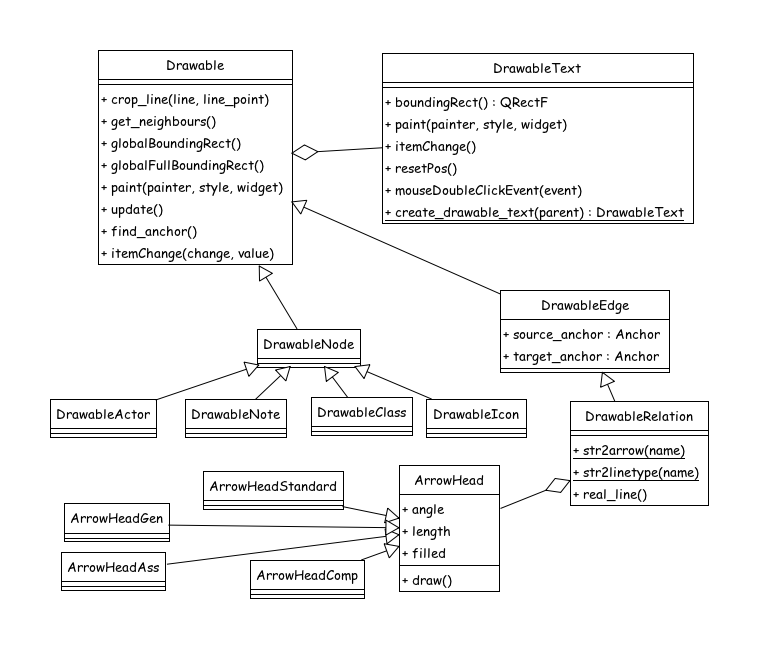
\includegraphics[width=\textwidth]{drawable}
  \end{center}
  \caption{Diagram klas modułu \texttt{modules}}
\end{figure}

\section{Działanie programu}
\subsection{Kompilacja}
% subsection

Kompilacja diagramów w programie \omlet składa się z następującego zestawu czynności:

\begin{itemize*}
  \item{Wczytanie kodu i jego wstępny podział na obiekty}
  \item{Sparsowanie kodu}
  \item{Uzupełnienie obiektów danymi z ich prototypów}
  \item{Odrzucenie prototypów}
  \item{walidacja skompilowanych obiektów}
\end{itemize*}

\subsubsection{Wczytanie kodu}
Za ten etap odpowiedzialna jest klasa \texttt{Code}.
Klasa przyjmuje napis, zawierający plik źródłowy.
Za pomocą klasy \texttt{Lexer} sprawdzane są kolejne linie.
Jeżeli linia jest definicją obiektu, tworzony jest nowy obiekt typu \texttt{\_CodeObject}, zawierający linie należące do obiektu następującego po znalezionym nagłówku.
Poza samymi liniami \texttt{\_CodeObject} przechowuje także informacje pozwalające określić numery linii w źródle.

Ponieważ pierwszy wiersz źródła nie musi być nagłówkiem obiektu, tworzony jest specjalny obiekt zerowy, przechowujące wszystkie linie przed pierwszym obiektem.

\subsubsection{Parsowanie kodu}
Obiekt klasy \texttt{Code}, zawierający obiekty \texttt{\_CodeObject} jest następnie przesyłany do klasy \texttt{Parser}.
Klasa ta zawiera funkcje budujące obiekty klasy \texttt{UMLObject}, na podstawie rozpoznanych symboli.
Obiekt klasy \texttt{Parser} Tworzy obiekt klasy \texttt{Lexer}, w którym zdefiniowana jest gramatyka.

Następnie metody klasy \texttt{Parser}, służące do budowania obiektów \texttt{UMLObject} są dodawane jako obiekty obsługujące symbole gramatyki.
Ostatecznie metoda \texttt{parse\_string} klasy \texttt{Lexer} zostaje wywołana i zostają utworzone obiekty \texttt{UMLObject} odpowiadające plikowi źródłowemu.

\subsubsection{Uzupełnienie obiektów}
Za uzupełnienie obiektów odpowiada obiekt klasy \texttt{DependencyResolver}.
Obiekt ten otrzymuje wszystkie obiekty \texttt{UMLObject}, które zostały stworzone w poprzednich krokach (oraz obiekty biblioteczne, tworzone przy inicjalizacji kompilatora).

Na początku obiekt sprawdza, czy nie występują cykliczne zależności pomiędzy obiektami (t.j. czy dwa lub więcej obiektów nie jest wzajemnie swoimi prototypami).

Następnie dla każdego obiektu znajdowany jest obiekt, będący jego prototypem i właściwości tego obiektu są dopisywane do aktualnego obiekt (pod warunkiem, że obiekt sam takich właściwości nie określa).

Po dojściu do obiektu, którego prototypem jest \texttt{base}, uzupełnianie danej gałęzi obiektów zostaje zakończone.

\subsubsection{Odrzucanie prototypów}
Prototypy muszą być odrzucone z puli obiektów z dwóch powodów:
\begin{itemize*}
  \item{Nie powinny być rysowane na diagramie}
  \item{Nie muszą być spójne} (spełniać wszystkich wymagań określonych przez ich prototypy). Pozostawienie ich przed następnym krokiem spowodowałoby niepotrzebne błędy.
\end{itemize*}

\subsubsection{Walidacja obiektów}
Obiekt klasy \texttt{Validator} sprawdza zgodność z danymi walidacji określonymi przez jego prototypy.

Normalnie sprawdzane jest istnienie, bądź nie istnienie konkretnej właściwości obiektu, oraz ew. zgodność typu tej właściwości.
Jeżeli prototypy określają wymagane wartości o typie \texttt{Object}, to sprawdzane jest także, czy wskazane przez te wartości obiekty istnieją.


\part{Instrukcja użytkownika}
\subsection{Okno programu}
Po uruchomieniu programu powinniśmy zobaczyć okno główne składające się z trzech paneli:

\begin{itemize}
	\item Edytor - panel służący do edycji aktualnie otwartego dokumentu.
	\item Podgląd - panel podglądu diagramu
	\item Lista błędów - sygnalizująca błędy w dokumencie
\end{itemize}

\subsection{Pasek menu oraz pasek narzędzi}
Opcje programu można wywoływać poprzez ikony na pasku narzędzi lub poprzez pasek menu.

Kolejno na pasku narzędzi znajdują się:
\begin{itemize}
	\item ,,New'' - otwiera nowy (pusty) dokument
	\item ,,Open document'' - otwiera istniejący dokument
	\item ,,Save'' - zapisuje aktualnie otwarty dokument
	\item ,,Save as'' - umożliwia zapisanie aktualnie otwartego dokumentu z wyborem nowej nazwy
	\item ,,Cut'' - funkcja ,,wytnij''
	\item ,,Copy'' - funkcja ,,kopiuj''
	\item ,,Paste'' - funkcja ,,wklej''
	\item ,,Undo'', ,,Redo'' - ,,cofnij'', ,,potwórz''
	\item ,,Generate'' - generuje diagram i wyświetla go w panelu podglądu
	\item ,,Export'' - zapisuje diagram widoczny w panelu podglądu do pliku obrazka
\end{itemize}

Dodatkowo na pasku menu znajduje się kategoria ,,Layout''. Menu ,,Layout'' służy do wyboru algorytmu rozkładania diagramów przy generacji. Do wyboru są różne algorytmy, zaleznie od platformy (a mianowicie obecności biblioteki \textbf{graphviz}).

\subsection{Praca z programem}

Zazwyczaj praca z programem rozpoczyna odczytania istniejącego dokumentu lub rozpoczęcia pracy nad nowym dokumentem - w drugim przypadku można zacząć pracować na pustym dokumencie który jest dostępny odrazu po otwarciu aplikacji. Użytkownik powinien najpierw zamodelować diagram opisująć jego strukturę, zgodnie z regułami języka, w panelu edycji diagramu. Następnie kliknięcie uzycie funkcji Generuj spowoduje wygenerowanie diagramu oraz wyświetlenie go w oknie podglądu. Nie stanie się tak w przypadku błędów krytycznych. Wszystkie błędy oraz ostrzeżenia sygnalizowane są w panelu błędów. Po wprowadzeniu poprawek do diagramu, można znowu kliknąć Generuj. W panelu podglądu powinniśmy wtedy zobaczyć uaktualniony diagram. W panelu podglądu możemy również przemieszczać elementy diagramu, wykonując gest ,,przeciągnij i upuść'' za pomocą myszy. Jeśli jesteśmy zadowoleni z diagramu, możemy użyć funkcji Eksportuj, która zapisze diagram do obrazka.

\section{Instrukcja użycia jezyka}

Głownym elementem języka jest \textbf{obiekt}. Obiekty mogą posiadać nazwę. Właściwości obiektu definiuje się za pomocą \textbf{par klucz-wartość}. Ważną właściwoscią obiektu jest nazwa obiektu bazowego, tj. obiektu który jest prototypem dla danego obiektu.

\begin{lstlisting}
class Klasa
	name: "Moja Klasa"
	stereotype: "Fajna"
\end{lstlisting}

Przykładem jest obiekt o nazwie ,,Klasa''. Jego prototypem jest obiekt o nazwie ,,class'', zdefiniowany w \textbf{bibliotece standardowej}. ,,Klasa'' posiada dwie pary klucz-wartość: ,,name'' oraz ,,stereotype''.

\subsection{Prototypy}

W powyższym przykładzie pokazaliśmy obiekt bazujący na obiekcie ,,class''. ,,class'' jest tzw. prototypem, zdefiniowanym następująco:

\begin{lstlisting}
prototype base class
    allow name STRING
    allow stereotype STRING
\end{lstlisting}

Słowo kluczowe \textbf{prototype} sprawi, że obiekt będzie ignorowany przez moduł rysujący diagram. Stanie się ,,niewidocznym obiektem'' używanym jako obiekt bazowy. \textbf{base} mówi, że obiekt nie bazuje na żadnym innym obiekcie. Deklaracje \textbf{allow} definiują ograniczenia nałożone na obiekty bazujące na tym prototypie. Sprawiają, ze bazując na ,,class'' będzie można ustawiać tylko klucze ,,name'' oraz ,,stereotype'' które mogą być typu \textbf{STRING} czyli ciąg znaków.

\subsubsection{Ograniczenia prototypów}

\emph{Uwaga - dalsza wiedza o prototypach nie jest potrzebna do wygodnego użytkowania programu.}

Oprócz \textbf{allow} można uzywać równiez \textbf{require}. \textbf{Require} sprawi, że użytkownik będzie zmuszony ustawić podany klucz, inaczej kompilacja diagramu nie powiedzie się.

Przykład \textbf{require}:
\begin{lstlisting}
prototype base relation
    require source-object OBJECT
    require target-object OBJECT
\end{lstlisting}

Poznaliśmy właśnie kolejny rodzaj wartości jaką można ustawić klucz - \textbf{OBJECT}. Wartość oczekiwana w tym wypadku to nazwa zdefiniowanego wcześniej obiektu, np. (ale niekoniecznie) prototypu.

Dozwolone ograniczenia na wartości to:
\begin{itemize}
	\item STRING - ciąg znaków
	\item OBJECT - nazwa zdefiniowanego obiektu
	\item MULTIPLICITY - UMLowa krotność, czyli liczba lub zakres, dozwolony znak *
	\item Lista wartości - lista dozwolonych identyfikatorów podawana w formacie: [a, b, c].
\end{itemize}

\subsubsection{,,Metody'' oraz ,,Atrybuty'' dla klas UML}

Język \omlet umożliwia definiowanie klas oraz atrybutów notacji UML. Wg przykładu:
\begin{lstlisting}
	+metoda(argument) : typ
    -atrybut : typ = "wartosc"
    _+statyczna_metoda()
\end{lstlisting}

\textbf{+} lub \textbf{-} przed nazwą metody/atrybutu oznacza widoczność (\emph{public} lub \emph{private}). \textbf{\_} przed widocznością pozwala zaznacza, że metoda jest statyczna. Po \textbf{:} można zdefiniować typ oraz, dla atrybutów, domyślną wartość.

\subsection{Dziedziczenie}

Tworząc obiekt bazujący na innym obiekcie (prototypie), obiekt przejmuje wszystkie ustawione klucze. Spójrzmy na przykład prototypu z ustawionymi kluczami:

\begin{lstlisting}
prototype relation generalization
    arrow: "generalization"
    direction: target
\end{lstlisting}

Teraz definiując obiekt bazujący na prototypie ,,generalization'', automatycznie przejmujemy wartości dla kluczy ,,arrow'' oraz ,,direction''. Znacznie ułatwia to tworzenie samych diagramów.

\subsection{Typy wbudowane}

Typem wbudowanym nazywamy obiekty które są interpretowane przez \omlet \footnote{A mianowicie moduł \textbf{DrawableFactory}} i potrafią być reprezentowane przez fizyczny \footnote{instancja pochodnych klasy Drawable} obiekt na diagramie. Dostępne typy wbudowane to:

\begin{itemize}
	\item actor
	\item class
	\item usecase
	\item note
	\item relation
\end{itemize}

Każdy z typów wbudowanych rysuje elementy diagramu używając zdefiniowanych kluczy. Biblioteka standardowa używa ograniczeń allow/require na kluczach uzywanych przez typy wbudowane w celu umożliwienia kompilatorowi sygnalizowania błędów.

\subsection{Prototypy dostępne w bibliotece standardowej}

Biblioteka standardowa udostępnia następujące prototypy używane do pisania diagramów. Obiekty bazowe odpowiadają wbudowanym typom, tzn. każdy obiekt bazowy ma swoją reprezentację na diagramach.

% SORRY ZA ITEMIZE MESS, NIE CHCIALO MI SIE ROBIC ADDCOMMAND BO NIE UMIEM DOBRZE :< MAM MAKRA W EDYTORZE.
\subsubsection{Actor}
Reprezentuje aktora UML.

Ograniczenia:
\begin{itemize}
	\item \textbf{name} (\emph{STRING}) Nazwa aktora. Wyświetlana pod symbolem aktora.
\end{itemize}
	
\subsubsection{Class}
Reprezentuje klasę UML.

Ograniczenia:
\begin{itemize}
	\item \textbf{name} (\emph{STRING}) Nazwa klasy.
	\item \textbf{stereotype} (\emph{STRING}) Stereotyp.
\end{itemize}

Typ wbudowany \textbf{class} zwraca uwagę na zdefiniowane \emph{metody i atrybuty UML}.

\subsubsection{Usecase}
Reprezentuje Use Case UML.

Ograniczenia:
\begin{itemize}
	\item \textbf{name} (\emph{STRING}) Nazwa przypadku użycia.
\end{itemize}

\subsubsection{Note}
Reprezentuje notatkę.

Ograniczenia:
\begin{itemize}
	\item \textbf{text} (\emph{STRING}) Tekst notatki
\end{itemize}
	
\subsubsection{Relation}
Relacja służąca do łączenia obiektów.

Ograniczenia:
\begin{itemize}
	\item \textbf{name} (\emph{STRING}) Nazwa relacji. Wyświetlana na środku odcinka łączącego obiekty.
	\item \textbf{arrow} Rodzaj strzałki. Dostępne strzałki to: ,,association'' ,,composition'' ,,aggregation'' ,,generalization''.
	\item \textbf{linetype} Rodzaj linii. Dostępne: ,,solid'', ,,dash'', ,,dot'', ,,dashdot''.
\end{itemize}

Dodatkowo \textbf{wymagane} (require) są: \textbf{target-object} oraz \textbf{source-object}, definiujące obiekty połączone relacją.

Definiować można również: \textbf{target-count} oraz \textbf{source-count} jako \emph{MULTIPLICITY} - są to krotności UML; \textbf{target-role} oraz \textbf{source-role} jako \emph{STRING} - są to role UML.

Kierunek relacji można zdefiniować na dwa sposoby: Ustawić \textbf{target-arrow} lub \textbf{source-arrow} na wybraną strzałkę (tak jak w kluczu \textbf{arrow}) lub użyć kluczy \textbf{arrow} (definiujący rodzaj strzałki) oraz \textbf{direction} przyjmujący [none, source, target, both], definiujący położenie strzałki.

Dodatkowo, zdefiniowane są następujące prototypy, bazujące na \textbf{relation}. Odpowiadają one danym relacją w notacji UML.
\begin{itemize}
	\item generalization
	\item association
	\item aggregation
	\item composition
\end{itemize}


\subsection{Przykłady uzycia języka}

Aplikacja potrafi wygenerować podstawowe elementy diagramu klas oraz diagramu przypadków użycia zdefiniowane w standardzie UML 2.0.

\subsubsection{Klasa}

Klasę definiuje się na podstawie prototypu \textbf{class}.\footnote{O prototypach będziem mowa w dalszej częsci}

\begin{lstlisting}
class Klasa
    stereotype : "Stereotyp"
    +metoda(argument) : typ
    -pole : typ = "wartosc"
    _+statyczna_metoda()
\end{lstlisting}
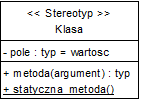
\includegraphics{klasa}
Utworzony został obiekt o identyfikatorze \textbf{Klasa}. Na diagramie będzie to nazwą klasy. Można również nadać inną nazwę korzystając z klucza \textbf{name}(którego nie ma w przykładzie). Klucz \textbf{stereotype} pełni rolę stereotypów w języku UML. Przykładowa klasa posiada metodę(wraz ze statyczną) oraz pole. Na uwagę zasługuje okreslenie widocznosci metod i pól: +, -, ~, \#. Statyczne metody lub pola oznacza się poprzez \_.
Mając już zdefiniowaną klasę \textbf{Klasa} można utworzyć na jej podstawie następny obiekt, kopiując wszystkie ustawione wartosci kluczy z \textbf{Klasa}: \textbf{Klasa} NewObject.

\subsubsection{Relacja}

Relację okresla się na podstawie prototypu \textbf{relation}.
\begin{lstlisting}
relation
    source-object : Aktor
    source-count : 1
    source-role : "Aktor"

    target-object : uc
    target-count : *
    name : "Uzywa"

actor Aktor
usecase uc
\end{lstlisting}
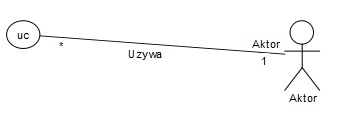
\includegraphics{relacja}
Relację jak wyżej można zdefiniować bez nazwy, jeżeli nie ma potrzeby wykorzystywać do tworzenia nowych obiektów pochodnych od relacji. Klucz \textbf{source-object} wskazuje obiekt na diagramie od którego relacja wychodzi, natomiast \textbf{target-object} wskazuje obiekt docelowy dla końca relacji. Klucze \textbf{source-role} oraz \textbf{target-role} odpowiadają za nadanie obiektowi źródłowemu i docelowemu ról zgodnie z notacją UML. Oczywiscie nazwa relacji na diagramie poprzez \textbf{name}. Ponadto relacja może zawierać klucze: \textbf{arror} odpowiadający za okreslenie rodzaju strzałki relacji oraz \textbf{direction}, który odpowiada za miejsce umieszczenia tej strzałki.

\subsubsection{Asocjacja}

Jako przykład asocjacji można użyć powyższy listing. Oczywiscie należałoby zmienić \textbf{relation} na \textbf{association}. Oparta jest również na odpowiednim prototypie. Asocjacja ma już na wstępie zdefiniowane klucze: \textbf{arrow} i \textbf{direction}. Można traktować asocjację jako podstawową formę relacji, tzn. bez kierunków.

\subsubsection{Generalizacja}

Jest relacją o okreslonym zwrocie i kierunku strzałki.
\begin{lstlisting}
generalization
    source-object : Aktor
    target-object: Klasa

actor Aktor
class Klasa
\end{lstlisting}
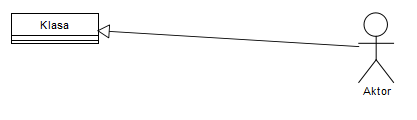
\includegraphics{generalizacja}

\subsubsection{Agregacja}

Różni się od generalizacji typem strzałki oraz jej kierunkiem.
\begin{lstlisting}
aggregation
    source-object : Klasa
    target-object: InnaKlasa

class InnaKlasa
class Klasa
\end{lstlisting}
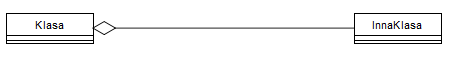
\includegraphics{agregacja}

\subsubsection{Kompozycja}

Kompozycja różni się od generalizacji i agregacji typem strzałki oraz ma kierunek zdefiniowany taki jak agregacja.
\begin{lstlisting}
composition 
    source-object : Aktor
    target-object : Notatka
    
actor Aktor
note Notatka
\end{lstlisting}
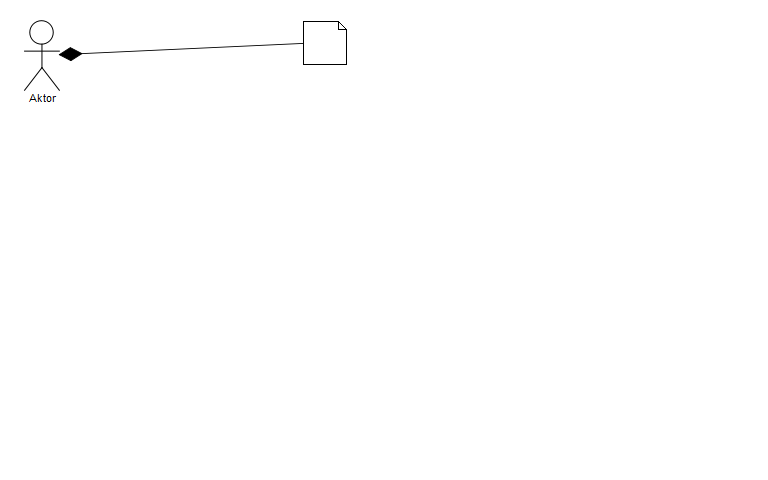
\includegraphics{kompozycja}

\subsubsection{Notatka}

Notatka może posiadać tylko tekst. Nie ma zdefiniowanych innych kluczy oprócz \textbf{text}.
\begin{lstlisting}
note 
    text : "Notatka Notatka Notatka Notatka Notatka Notatka Notatka Notatka"
\end{lstlisting}
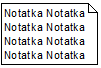
\includegraphics{notatka}

\subsubsection{Aktor i przypadek użycia}

Aktor posiada tylko klucz \textbf{name}. Podobnie przypadek użycia.
\begin{lstlisting}
actor Aktor

usecase uc
    name : "Przypadek uzycia"
\end{lstlisting}
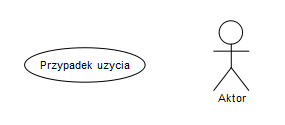
\includegraphics{aktor_uc}

\end{document}
